% J'utilise Latex Workshop sur VSCODE pour compiler et générer le pdf depuis un fichier Latex comme celui ci
% lien d'une vidéo permettant de le DL : https://www.youtube.com/watch?v=4lyHIQl4VM8

\documentclass{article}

\usepackage{amsmath,amsthm,amsfonts,amssymb,amscd} % package mathématiques permettant de faciliter l'utilisation de symboles mathématiques et de théorèmes
\usepackage{tikz-cd} % package permettant de faire des graphs
\usepackage{fancyhdr} % permet de personnaliser l'entete et le pied de page
\usepackage[margin=3cm]{geometry} % permet de gérer les marges et dimensions de la page
\usepackage[latin1]{inputenc} % aucune idée mais ca marche pas sans lui
\usepackage[english]{babel} % permet l'utilisation d'un sommaire
\usepackage{hyperref} % permet que le sommaire redirige
\usepackage{graphicx} % permet d'ajouter des images
\usepackage[nottoc]{tocbibind} % permet d'ajouter la page de garde dans le sommaire
\setlength{\parindent}{0pt}

% ------ en tête ------
\geometry{margin=1in, headsep=0.5in}
\pagestyle{fancy}
\setlength{\headheight}{10pt}
\lhead{\textcolor{red}{\Huge ISEN Nantes}}  
\rhead{Graph Theory}
\begin{document}
\title{Graph Theory - Graphs}

% ------ Page de Garde------

% ----- Page de Garde -----

\begin{center}
    
\includegraphics[width=0.35\textwidth]{image/ISEN.png}\\
\end{center}
    \rule{\linewidth}{0.5mm}
        
    \begin{center}
        {\Huge \bf Final Project}
    \end{center}
    
    \begin{center}
        {\LARGE \bf The Maximum Edge Weight Clique Problem}
    \end{center}
    \rule{\linewidth}{0.5mm}
    
    \vspace{1\baselineskip}
    
    \begin{center}
    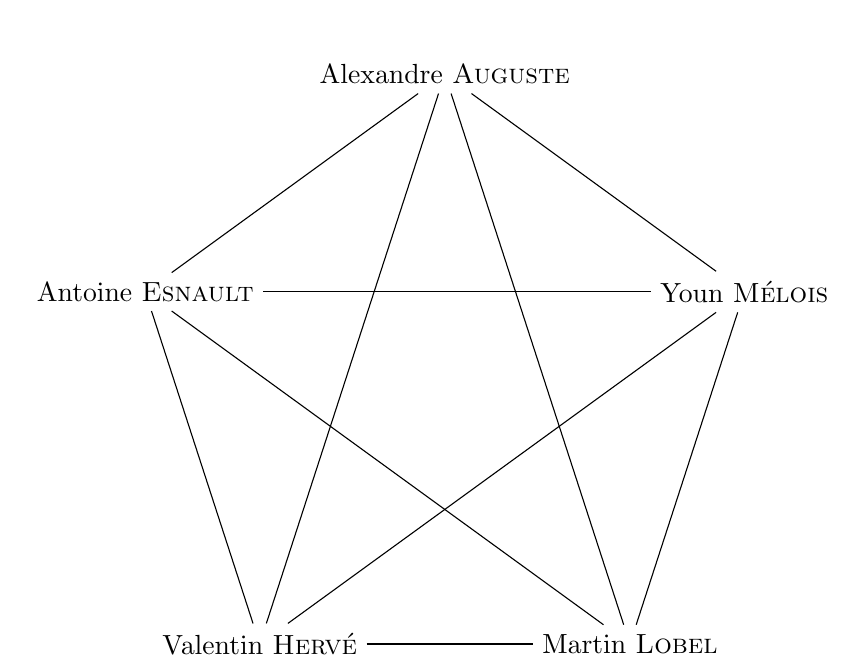
\begin{tikzpicture}[commutative diagrams/every diagram]
        \node (P0) at (90:4cm) {Alexandre \textsc{Auguste}};
        \node (P1) at (90+72:4cm) {Antoine \textsc{Esnault}} ;
        \node (P2) at (90+2*72:4cm) {Valentin \textsc{Herv\'e}};
        \node (P3) at (90+3*72:4cm) {Martin \textsc{Lobel}};
        \node (P4) at (90+4*72:4cm) {Youn \textsc{M\'elois}};
        \path
        (P0) edge node {} (P1)
        (P0) edge node {} (P2)
        (P0) edge node {} (P3)
        (P0) edge node {} (P4)
        (P1) edge node {} (P2)
        (P1) edge node {} (P3)
        (P1) edge node {} (P4)
        (P2) edge node {} (P3)
        (P2) edge node {} (P4)
        (P3) edge node {} (P4);
    \end{tikzpicture}
    \end{center}
    \vspace{1\baselineskip}   
    \large \textbf{Abstract} The Maximum Edge Weight Clique (MEWC) problem is an optimization problem in graph theory that asks for the clique (a subset of vertices, all adjacent to one another) with the maximum total weight in an edge-weighted undirected graph. In the MEWC problem, each edge has a weight, and the weight of a clique is the sum of the weights of its edges. The goal is to find a clique with the maximum possible weight. 

    \begin{center} \Large
        \emph{Class group :}\\
        \textsc{CIR3} - Team 1 \\
    \end{center}
    
    \begin{center} \Large
        \emph{Teacher :}\\
        Leandro \textsc{Montero}
    \end{center}
    
    \vfill
    
\begin{center} \Large
        \today
\end{center}
    
\newpage

% ------ Sommaire ------

\tableofcontents
\newpage

% ------ Introduction ------
% jsp si il faut que je la remette mais osef, ca présente le projet

% ----- Introduction -----

\section{Introduction}

\subsection{Presentation of the subject}

\textbf{Graph theory} is a branch of mathematics that deals with the study of graphs,
which are mathematical structures used to model pairwise relationships between
objects. Graphs consist of vertices (also called nodes) that are connected by
edges. The edges can be either directed (one-way) or undirected (two-way) and can
also have a weight. \newline

\textbf{The Maximum Edge Weight Clique} (MEWC) problem is an optimization problem
in graph theory that asks for the clique (a subset of vertices, all adjacent to
one another) with the maximum total weight in an edge-weighted undirected graph.
In the MEWC problem, each edge has a weight, and the weight of a clique is the
sum of the weights of its edges. The goal is to find a clique with the maximum
possible weight. \newline

Now, the MEWC problem is \textbf{NP-hard}, which means that it is not possible
to find an efficient algorithm to solve it in polynomial time or that this problem
is at least as hard as the hardest problems in NP. It is also the generalization
of the Maximum Clique Problem (MCP), which is the special case where all edges
have the same weight. \newline

\begin{minipage}{0.5\textwidth}
    For example, the following graph $G=(V,E)$ has for its set of vertices
    $V=\{1,2,3,4,5,6\}$ and for its set of edges
    $E=\{(1,2),(1,5),(2,3),(2,5),(3,4),(4,5),(4,6)\}$.
    As we can see, the red edges form a clique of size 3 and the other colored
    edges are each cliques of size 1. We can also easily deduct that the maximum
    clique of G is the red clique of size 3.
\end{minipage}
\begin{minipage}{0.5\textwidth}
    \begin{figure}[H]
        \centering
        \begin{tikzpicture}[node distance=2cm]
            \node (1) {1};
            \node (2) at ([shift=(210:2)] 1) {2};
            \node (3) [left of=2] {3};
            \node (4) [above of=3] {4};
            \node (5) [above of=2] {5};
            \node (6) at ([shift=(150:2)] 4) {6};

            \draw[red] (1) -- (2);
            \draw[red] (1) -- (5);
            \draw[green] (2) -- (3);
            \draw[red] (2) -- (5);
            \draw[blue] (3) -- (4);
            \draw[orange] (4) -- (5);
            \draw[cyan] (4) -- (6);
        \end{tikzpicture}
        \caption{Basic graph example}
    \end{figure}
\end{minipage} \\ \\

The MEWC problem can be used to model various types of real-world situations where
the goal is to find a subset of objects with the maximum total weight, and the
objects are connected by weighted edges. Here are a few examples of such situations:

\begin{itemize}
    \item \textbf{Network design}: In a communication network, the MEWC problem
          can be used to find the optimal subset of devices (vertices) to include in
          the network, such that the total cost of communication between the devices
          (edges) is maximum.
    \item \textbf{Protein interaction}: In biology, the MEWC problem can be used
          to find the optimal subset of proteins (vertices) in a protein-protein
          interaction network, such that the total interaction strength (edges)
          between the proteins is maximum.
    \item \textbf{Social network analysis}: In a social network, the MEWC problem
          can be used to find the optimal subset of individuals (vertices) with
          the maximum total relationship strength (edges) between them.
\end{itemize}

% ----- Configuration -----

\subsection{Configuration}

-  Ajouter les configurations que l'on a utilise pour les tests du style la config\\ \\

On this project, we decide to use \textbf{the C++ language} to developp and implement our algorithms. Nevertheless, a debate took place, especially on the choice of the language. We hesitated between Python and C++. The first one was for us easier to handle and was a tool in which we had more confidence in our ability to use it efficiently. The latter was nevertheless preferred because of its speed of execution, which was an important criterion for the study. We did have some problems with memory allocation, which made us regret this choice at times.  \\ \\
To share the code between us, we used \textbf{Github}\footnotemark \footnotetext{\url{https://github.com/sehnryr/Final-Graph-Project-ISEN-CIR3}}. It is a web-based platform for version control, collaboration, and sharing of code, as well as a community of developers who contribute to open source projects and share their knowledge. It was a tool that was difficult for some to get used to quickly, especially on the configuration of the project at home, but which brought us a significant gain in efficiency once we had understood how to use it. To share information and communicate between us, we used \textbf{Discord}.



% ----- Applications -----

\subsection{Example of real-life situations}

As we said, the MEWC has many real-life applications in various fields such as social networks, chemistry, bioinformatics. We could model this problem with some fast example like these :
\begin{itemize}
    \item We can model this problem on social \textbf{social networks}, indeed we can represent each \textbf{users} as a \textbf{vertex} in a graph and add an \textbf{edge} between two vertices if the corresponding individuals \textbf{have some kinds of relationships together}. The weight of the edge could represent \textbf{the degree of relationships} between the two users. The goal here is to identify the group of individuals with the strongest connections within a social network. Some example can be Twitter or Netflix.
    \item Furthermore, we can model the MEWC problem on \textbf{chemistry}, indeed we can represeant each \textbf{chemical compounds} as a \textbf{vertex} in a graph and add an \textbf{edge} between two vertices if the corresponding chemical compounds \textbf{have an intermolecular interaction between them}. The weight of the edge could represent the \textbf{he strength of the corresponding intermolecular interaction}. The goal here is to identify the compound with the strongest intermolecular interactions from a set of potential drug candidates. Some example can be found on research.
\end{itemize}
We will take a practical example which could include and involve ISEN students in our future. We will reuse the presented case to illustrate the different algorithms that we will implement later in the report.\\ \\
\textbf{An example of real-life situations that can be modelled as MEWC} is \ul{the team formation process} during a project, or in the search for a particular social group.
\\ \\
We can imagine that the Student Office of ISEN Nantes is looking to reinforce the video games club of its school. Indeed, the latter has no succession for the following year and is thus led to die if no member presents himself. The future members of the office will have to be in contact with each other during a whole year and it is thus important to find people with common interests so that no tension is formed during their studies. The office has access to the Steam profiles of the students within ISEN (Steam is a video game digital distribution service that gives information about the games played by each one) as well as a record made by the gaming club of the different games played by their members. The fact of playing games in common could bring some people closer, and this makes it a good criterion to create a group that could take over the club because it would share common interests. Otherwise, it would allow to see which games and which group could be present at different events they could organize. Here, forming a team from a group of individuals can be considered as a maximum edge weight clique problem because the goal is to select a subset of individuals such that the members share a common interest.
\\ \\
To model this problem as a maximum edge weight clique problem, we can represent each \textbf{individual} as a \textbf{vertex} in a graph and add an \textbf{edge} between two vertices if the corresponding individuals \textbf{share atleast one game}. The weight of the edge could represent \textbf{the number of game} that they have in common.
\\ \\
For example, on a small scale we could imagine :
\\ \\
\begin{tabular}{|p{0.3\textwidth}|p{0.65\textwidth}|}
    \hline
    \textbf{Students} & \textbf{Game played}                         \\
    \hline
    Youn              & Minecraft, Civilisations, Lost ARK, Among US \\
    \hline
    Martin            & Minecraft                                    \\
    \hline
    Valentin          & Genshin, Minecraft, Civilisations            \\
    \hline
    Bastien           & Genshin, Minecraft, Lost ARK, Among US       \\
    \hline
    Guillaume         & CSGO, Genshin, Overwatch, Stardew Valley     \\
    \hline
    Dorian            & CSGO, Paladins, Overwatch                    \\
    \hline
    Antoine           & League of Legends, Stardew Valley            \\
    \hline
    Thomas            & League of Legends, The Last of US            \\
    \hline
    Alexandre         & League of Legends, Dofus                     \\
    \hline
\end{tabular}
\vspace{1\baselineskip} \\
Which would give us this graph :

\begin{center}
    \begin{tikzcd}
        Youn \arrow[dd, dash, "1"] \arrow[r, dash, "2"] \arrow[ddr, dash, "3"] & Valentin \arrow[r, dash, "1"] \arrow[ddl, dash, "1"] \arrow[dd, dash, "2"] & Guillaume \arrow[ddl, dash, "1"] \arrow[dd, dash, "2"] \arrow[r, dash, "1"] & Antoine \arrow[dd, dash, "1"] \arrow[dr, dash, "1"] \\
        & & & & Alexandre \\
        Martin \arrow[r, dash, "1"] & Bastien & Dorian & Thomas \arrow[ur, dash, "1"]
    \end{tikzcd}
\end{center}

The goal of the maximum edge weight clique problem in this context would be to find a complete subset of individuals such that the sum of the weights of the edges between the individuals is maximized. In this example, the maximum weight clique would be the clique consisting of nodes Youn, Valentin, Martin, Maxence with a total weight of $10(2+1+1+1+3+2)$.

% Indeed, we could imagine that Nils Baussé need to make a team for a robotic event in Nantes during the hollidays. As the students of CIR3 do not all live in Nantes during their vacation period, he needs to form a group that is geographically close to each other so that they can meet quickly, do tests and participate in the event to present the project. Here, forming a team from a group of individuals can be considered as a maximum edge weight clique problem because the goal is to select a subset of individuals in order to optimize the global location of the team.
% \newline

% To model this problem as a maximum edge weight clique problem, you can represent each individual as a node in a graph and add an edge between two nodes if the corresponding individuals are located within 10 km of each other. The weight of the edge could represent a number proportional to the distance between the two people. The closer they are, the bigger the number would be and the further they are, the smaller the number would be. We will take the weight $w$ as : $$w = \frac{1}{\text{distance between the two individuals}} \times 100$$
% \newline

% For example, we could imagine that Youn lives 7km away from Martin, the weigth between these two will be : $$w_{Youn/Martin} = \frac{1}{7} \times 100 = 14.3$$
% \newline
% \begin{center}
%     \begin{tikzcd} 
%         Youn \arrow[dd, dash, "14.3"] \arrow[r, dash, "23"] \arrow[ddr, dash, "43"] & Valentin \arrow[r, dash, "70"] \arrow[ddl, dash, "15"] \arrow[dd, dash, "100"] & Aubin \arrow[ddl, dash, "85"] \arrow[dd, dash, "15"] \arrow[r, dash, "13"] & Antoine \arrow[dd, dash, "12"] \arrow[dr, dash, "10"] \\
%         & & & & Alexandre \\
%         Martin \arrow[r, dash, "16"] & Maxence & Dorian & Thomas \arrow[ur, dash, "12"]
%     \end{tikzcd} 
% \end{center}

% The goal of the maximum edge weight clique problem in this context would be to find a subset of individuals such that the sum of the weights of the edges between the individuals is maximized. In this example, the maximum weight clique would be the clique consisting of nodes Valentin, Aubin, Maxence with a total weight of $255(100+170+85)$.

\newpage

% ----- Exact Algorithm -----

% ----- Exact Algorithm -----

\section{Exact Algorithm}

% ----- Presentation -----

\subsection{Presentation}

An exact algorithm for solving the MEWC problem works by exploring all potential
cliques in the graph and selecting the clique with the maximum weight. To do this,
the algorithm uses a recursive function to explore all possible subsets of V.
For each subset, the algorithm computes the weight of the clique formed by the
vertices in the subset. If the weight is greater than the current maximum weight,
the clique is selected as the current maximum. This process is repeated until all
possible cliques have been explored, at which point the algorithm returns the
clique the the maximum weight.
\newline \newline
The time complexity of this approach is $\mathcal{O}(n^2\times2^n)$, where $n$ 
is the number of vertices in the graph. This is due to the fact that there are 
$2^n$ possible subsets of V, and the algorithm must compute the weight of the clique, 
which by itself has a complexity of $\mathcal{O}(n^2)$ because there are at most
$\frac{n(n-1)}{2}$ edges in a complete graph, and compare it to the current 
maximum weight. Therefore, the algorithm is only feasible for small-scale graphs.
\newline \newline
However, there is a better algorithm called the \textbf{Bron-Kerbosch}
algorithm\cite{finding-all-cliques-of-an-undirected-graph} that can find all 
maximal cliques in a graph with a time complexity of $\mathcal{O}(3^{\frac{n}{3}})$, 
where $n$ is the number of vertices in the graph. 
This algorithm is optimal, as it has been proven by J. W. Moon \& L. Moser in 
1965\cite{on-cliques-in-graphs} that there are at most $3^{\frac{n}{3}}$ maximal 
cliques in any n-vertex graph.
\newline \newline
We can use the Bron-Kerbosch algorithm to find all maximal cliques in the graph,
and then compute the weight of each clique. This approach has a time complexity of
$\mathcal{O}(n^2\times3^{\frac{n}{3}})$, which is much better than the previous
approach. However, this algorithm is still not feasible for large-scale graphs.

% ----- Fonctionnement -----

\subsection{How it works}

    As said before, our algorithm first uses Bron-Kerbosc to obtain all the maximal cliques of the input graph. Then, it looks for which cliques have the highest weight. So we will explain how it does to get the different maximal cliques. \\

    The Bron-Kerbosch pivot algorithm that we used is a more efficient variant of the Bron-Kerbosch algorithm that is used to find all the cliques in a graph. It works in a similar way to the original Bron-Kerbosch algorithm, but uses a pivot vertex to guide the search for cliques. \\

    At each step of the algorithm, the pivot algorithm keeps track of three groups of vertices: the candidates, which are the set $P$ of vertices that could potentially be part of the clique, the already-selected vertices, which are the set $R$ of vertices that are definitely part of the clique, and the set $X$ of vertices that have been considered but not selected. \\

    The algorithm selects a pivot vertex from the set of candidates and already-selected vertices, and then adds to the candidate set any vertices that are connected to all of the vertices in the already-selected set, as well as the pivot vertex. It then removes from the candidate set any vertices that are not connected to all of the vertices in the already-selected set, and adds those vertices to the set X of vertices that have been considered but not selected. \\

    This process is repeated until the candidate set is empty. At that point, all of the vertices in the already-selected set form a clique. The algorithm is then run again on the remaining candidates and already-selected vertices to find any additional cliques. \\

    We will now illustrate it step by step with a practical example : \\

    \hspace*{1cm} \textbf{Step 0 :}
    \\
    \begin{minipage}{0.4\textwidth}
        \begin{tikzcd}
            6 \arrow[r, dash] & 4 \arrow[r, dash] \arrow[dd, dash] & 5 \arrow[dr, dash] \arrow[dd, dash] \\
            & & & 1 \\
            & 3 \arrow[r, dash] & 2 \arrow[ur, dash]
        \end{tikzcd}
    \end{minipage}
    \begin{minipage}{0.6\textwidth}
        We have here our graph as an example. As said before, the Bron-Kerbosh pivot algorithm will take 3 parameters. $R$, the set of vertices already selected. $P$, the set of candidate vertices. $X$, the set of vertices that have been considered but not selected.
    \end{minipage}
    Here, we have :
    $$ \boxed{
            \begin{array}{lll}
                R = \{\} & P = \{1,2,3,4,5,6\} & X = \{\} \\
            \end{array}
    }$$
    \\ 
    \hspace*{1cm}  \textbf{Step 1 :}
    \\
    \begin{minipage}{0.4\textwidth}
        \begin{tikzcd}
            6 \arrow[r, dash] & 4 \arrow[r, dash] \arrow[dd, dash] & 5 \arrow[dr, dash] \arrow[dd, dash] \\
            & & & 1 \\
            & 3 \arrow[r, dash] & \color{red} 2 \arrow[ur, dash]
        \end{tikzcd}
    \end{minipage}
    \begin{minipage}{0.6\textwidth}
        Now, to begin the algorithm, we will need to chose a pivot $u$. The pivot $u$ should be chosen as one of the degree-three vertices, to minimize the number of recursive calls. Now, we suppose that $u$ is chosen to be vertex 2. We see, that there is 2 vertices that are not adjacent to 2 which are 4 and 5.
    \end{minipage}
    Then we know that we will work by starting with these 3 configurations (we know the first, but we don't know yet for the vertex $4$ and $6$ because some vertex could be added to $X$ or removed from $P$ when we process on $2$ or $4$) :
    $$ \boxed{
        \begin{array}{lll}
            R = \{2\} & P = \{1,3,5\} & X =\{\}\\
            R = \{4\} \\
            R = \{6\} \\
        \end{array}
    }$$
    \\
    \hspace*{1cm}  \textbf{Step 2 :}
    \\
    \begin{minipage}{0.4\textwidth}
        \begin{tikzcd}
            6 \arrow[r, dash] & 4 \arrow[r, dash] \arrow[dd, dash] & \color{green} \textcircled{5} \arrow[dr, dash] \arrow[dd, dash] \\
            & & & \color{green} \textcircled{1} \\
            & \color{green} 3 \arrow[r, dash] & \color{red} \textcircled{2} \arrow[ur, dash]
        \end{tikzcd}
    \end{minipage}
    \begin{minipage}{0.6\textwidth}
        The algorithm begins by looking at vertex 2 in the graph. It makes a recursive call with using vertex 2 as a starting point. In this recursive call, the algorithm looks at the first group of vertices it was given (vertices 1 and 5) and selects one of them as the pivot vertex. Let's say it selects vertex 1. It then makes a first second-level recursive call for vertex 5. That will eventually find the clique $(1,2,5)$.
    \end{minipage}
    The recursive call process like this  :
    $$ \boxed{
        \begin{array}{lll}
            R = \{2\} & P = \{1,3,5\} & X = \{\} \\
            R = \{2,5\} & P = \{1\} & X = \{\} \\
            R = \{2,5,1\} & P = \{\} & X = \{\} \\
        \end{array} 
        \rightarrow P = \O \text{ and } X = \O \text{ then } (2,5,1) \text{ is a clique.}
    }$$
    \\
    \\
    \begin{minipage}{0.4\textwidth}
        \begin{tikzcd}
            6 \arrow[r, dash] & 4 \arrow[r, dash] \arrow[dd, dash] & \color{green} 5 \arrow[dr, dash] \arrow[dd, dash] \\
            & & & \color{green} 1 \\
            & \color{green} \textcircled{3} \arrow[r, dash] & \color{red} \textcircled{2} \arrow[ur, dash]
        \end{tikzcd}
    \end{minipage}
    \begin{minipage}{0.6\textwidth}
        The algorithm then makes a second second-level recursive calls for vertex 3. That will eventually find the clique $(2,3)$. After these two second level recursive calls have completed, vertex 2 is added to X and removed from P.
    \end{minipage}
    The recursive call process like this  :
    $$ \boxed{
        \begin{array}{lll}
            R = \{2\} & P = \{1,3,5\} & X = \{\} \\
            R = \{2,3\} & P = \{\} & X = \{\} \\
            R = \{\} & P = \{1,3,4,5,6\} & X = \{2\} \\
        \end{array} 
        \rightarrow P = \O \text{ and } X = \O \text{ then } (2,3) \text{ is a clique.}
    }$$
    \\
    \hspace*{1cm}  \textbf{Step 3 :}
    \\
    \begin{minipage}{0.4\textwidth}
        \begin{tikzcd}
            \color{green} 6 \arrow[r, dash] & \color{red} \textcircled{4} \arrow[r, dash] \arrow[dd, dash] & \color{green} 5 \arrow[dr, dash] \arrow[dd, dash] \\
            & & & 1 \\
            & \color{green} \textcircled{3} \arrow[r, dash] & 2 \arrow[ur, dash]
        \end{tikzcd}
    \end{minipage}
    \begin{minipage}{0.6\textwidth}
        it will now do an iteration taking 4 as vertices. We note that the vertex 2 belongs to the set X in the outer call to the algorithm, but it is not a neighbor of the vertex 4 and is excluded from the subset of X passed to the recursive call. The algorithm makes a first second-level recursive call for vertex 3. That will eventually find the clique (3, 4).
    \end{minipage}
    The recursive call process like this  :
    $$ \boxed{
        \begin{array}{lll}
            R = \{4\} & P = \{3,5,6\} & X = \{\} \\
            R = \{4,3\} & P = \{\} & X = \{\} \\
        \end{array} 
        \rightarrow P = \O \text{ and } X = \O \text{ then } (4,3) \text{ is a clique.}
    }$$
    \\
    \begin{minipage}{0.4\textwidth}
        \begin{tikzcd}
            \color{green} 6 \arrow[r, dash] & \color{red} \textcircled{4} \arrow[r, dash] \arrow[dd, dash] & \color{green} \textcircled{5} \arrow[dr, dash] \arrow[dd, dash] \\
            & & & 1 \\
            & \color{green} 3 \arrow[r, dash] & 2 \arrow[ur, dash]
        \end{tikzcd}
    \end{minipage}
    \begin{minipage}{0.6\textwidth}
        The algorithm makes a second second-level recursive call for vertex $5$. That will eventually find the clique $(4,5)$.
    \end{minipage}
    The recursive call process like this  :
    $$ \boxed{
        \begin{array}{lll}
            R = \{4\} & P = \{3,5,6\} & X = \{\} \\
            R = \{4,5\} & P = \{\} & X = \{\} \\
        \end{array} 
        \rightarrow P = \O \text{ and } X = \O \text{ then } (4,5) \text{ is a clique.}
    }$$
    \\
    \begin{minipage}{0.4\textwidth}
        \begin{tikzcd}
            \color{green} \textcircled{6} \arrow[r, dash] & \color{red} \textcircled{4} \arrow[r, dash] \arrow[dd, dash] & \color{green} 5 \arrow[dr, dash] \arrow[dd, dash] \\
            & & & 1 \\
            & \color{green} 3 \arrow[r, dash] & 2 \arrow[ur, dash]
        \end{tikzcd}
    \end{minipage}
    \begin{minipage}{0.6\textwidth}
        The algorithm makes a third second-level recursive call for vertex $6$. That will eventually find the clique $(4, 6)$. After these three second level recursive calls have completed, vertex 4 is added to X and removed from P.
    \end{minipage}
    The recursive call process like this  :
    $$ \boxed{
        \begin{array}{lll}
            R = \{4\} & P = \{3,5,6\} & X = \{\} \\
            R = \{4,6\} & P = \{\} & X = \{\} \\
            R = \{\} & P = \{1,3,5,6\} & X = \{2,4\} \\
        \end{array} 
        \rightarrow P = \O \text{ and } X = \O \text{ then } (4,6) \text{ is a clique.}
    }$$
    \\
    \hspace*{1cm}  \textbf{Step 4 :}
    \\
    \begin{minipage}{0.4\textwidth}
        \begin{tikzcd}
            \color{red} \textcircled{6} \arrow[r, dash] & \textcircled{x} \arrow[r, dash] \arrow[dd, dash] & 5 \arrow[dr, dash] \arrow[dd, dash] \\
            & & & 1 \\
            & 3 \arrow[r, dash] & 2 \arrow[ur, dash]
        \end{tikzcd}
    \end{minipage}
    \begin{minipage}{0.6\textwidth}
        It will now do a third and final iteration taking 6 as vertex. It makes a recursive call but because $P$ is empty and $X$ is nom empty (the vertex $4$ was added to X and removed from P in step 3). Because of that, the algorithm immediately stops searching for cliques and backtracks, because there can be no maximal clique that includes the  vertex 6 and excludes the vertex 4.
    \end{minipage}
    The recursive call process like this  :
    $$ \boxed{
        \begin{array}{lll}
            R = \{6\} & P = \{\} & X = \{4\} \\
        \end{array} 
        \rightarrow \text{ No clique was found}
    }$$
    \\
    The algorithm is therefore \textbf{finished}, and we have obtained the cliques :
    $$\{(2,3),(1,2,5),(3,4),(4,5),(5,6)\}$$ 

    To summarize things and try to make things even clearer, we will take another example and make the call tree of it (the precedent example is too big) :

    \begin{center}
        \begin{tikzcd}
            1 \arrow[rr, dash] \arrow[dr, dash] & & 3 \arrow[rr, dash] \arrow[dl, dash] & & 4 \\
            & 2 & & 5
        \end{tikzcd}
    \end{center}
    His call tree :
    \begin{center}
        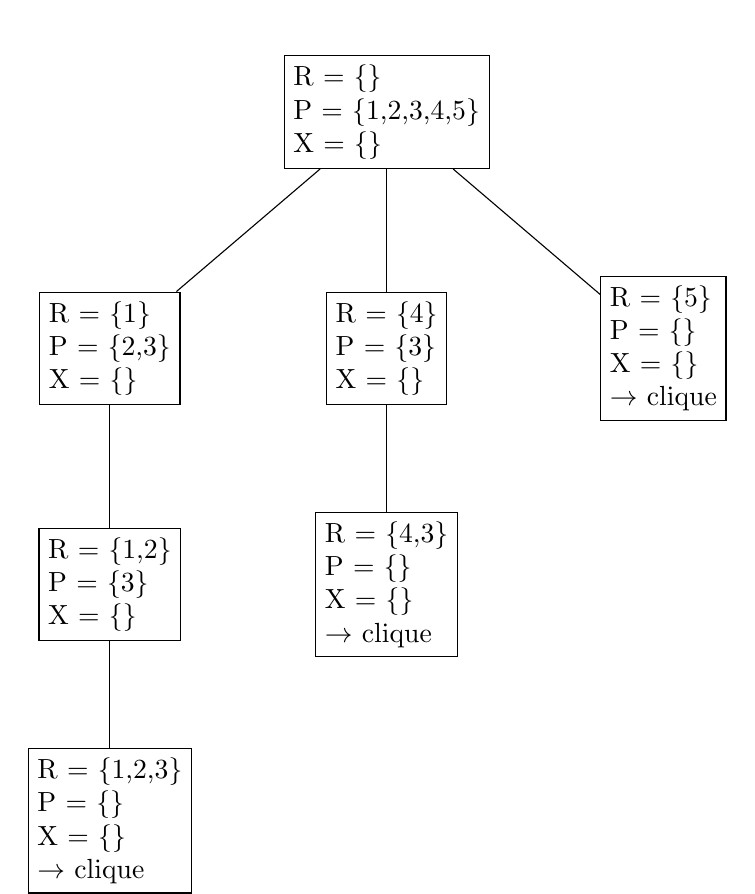
\begin{tikzpicture}[sibling distance=10em, level distance=30mm, every node/.style = {shape=rectangle, draw, align=left, top color=white}]
            \node {
                R = \{\} \\
                P = \{1,2,3,4,5\} \\
                X = \{\} 
            }
            child { node {
                R = \{1\} \\
                P = \{2,3\} \\
                X = \{\} 
            }
                child { node {
                    R = \{1,2\} \\
                    P = \{3\} \\
                    X = \{\} 
                }
                child { node {
                        R = \{1,2,3\} \\
                        P = \{\} \\
                        X = \{\} \\
                        $\rightarrow$ clique 
                }
            }}}
            child { node {
                R = \{4\} \\
                P = \{3\} \\
                X = \{\} 
            }
                child { node {
                        R = \{4,3\} \\
                        P = \{\} \\
                        X = \{\} \\
                        $\rightarrow$ clique 
            }}}
            child { node {
                R = \{5\} \\
                P = \{\} \\
                X = \{\} \\
                $\rightarrow$ clique
            }};
          \end{tikzpicture}
    \end{center}

    After getting every clique, the exact algorithm will iterate all maximal clique and apply a function that will return the total weight of it. 
    \\ \\
    This function work by iterating every possible pairs of vertices in the clique and the weight of it if there is an edge between them in a variable that start at 0. The variable will be returned as the total weight of the clique.   
    \\ \\
    Some quick example of it :
    \\ \\
    \hspace*{1cm}  \textbf{Step 1 :} 
    
    \begin{center}
        Total Weight $= 0$ (start)
    \end{center}
  
    \begin{minipage}{0.4\textwidth}
        \begin{tikzcd}
            & \color{red} 1 \arrow[dl, dash, red, "3"] \arrow[dr, dash, "4"] \\
            \color{red} 2 \arrow[rr, dash, "1"] & & 3
        \end{tikzcd}
    \end{minipage}
    \begin{minipage}{0.6\textwidth}
        The function will take the vertex $1$ and $2$, the edge between them have a weight of $3$. It will add 3 in the variable "Total Weight". 
    \end{minipage}
    \begin{center}
        Total Weight $= 0 + 3 = 3$
    \end{center}
    
    \hspace*{1cm}  \textbf{Step 2 :}
    \\
    \begin{minipage}{0.4\textwidth}
        \begin{tikzcd}
            & 1 \arrow[dl, dash, "3"] \arrow[dr, dash, "4"] \\
            \color{red} 2 \arrow[rr, dash, "1", red] & & \color{red} 3
        \end{tikzcd}
    \end{minipage}
    \begin{minipage}{0.6\textwidth}
        The function will take the vertex $2$ and $3$, the edge between them have a weight of $1$. It will add 1 in the variable "Total Weight".
    \end{minipage}
    \begin{center}
        Total Weight $= 3 + 1 = 4$
    \end{center}
    
    \hspace*{1cm}  \textbf{Step 3 :}
    \\
    \begin{minipage}{0.4\textwidth}
        \begin{tikzcd}
            & \color{red} 1 \arrow[dl, dash, "3"] \arrow[dr, dash, red, "4"] \\
            2 \arrow[rr, dash, "1"] & & \color{red} 3
        \end{tikzcd}
    \end{minipage}
    \begin{minipage}{0.6\textwidth}
        The function will take the vertex $1$ and $3$, the edge between them have a weight of $4$. It will add 4 in the variable "Total Weight".
    \end{minipage}
    \begin{center}
        Total Weight $= 4 + 4 = 8$
    \end{center}

    The total weight of this clique is 8.
    \\ \\
    The algorithm then takes the clique with the greatest weight. And \textbf{the MEWC is solved}.

% ----- Pseudo - Code -----

\subsection{Pseudo code}

% ----- Complexité -----

\subsection{Complexity}

% ----- Bad Instance -----

\subsection{Bad Instance}
    
    The exact algorithm have no bad instance, he will always find the optimal solution each time. However, it will take a fairly long time to do so.

% ----- Experiments -----

\subsection{Experiments}

% ----- Analyse -----

\subsection{Analysis}

\newpage

% ----- Constructive Algorithm -----

% ----- Constructive Algorithm -----

\section{Constructive Algorithm}

% ----- Presentation -----

\subsection{Presentation}

    A \textbf{heuristic algorithm} is a type of algorithm that uses rules of thumb to try to find an approximate solution to a problem, rather than an exact one. Heuristic algorithms are often used when it is not possible to find an exact solution to a problem, or when an exact solution would be too time-consuming to compute. They are also used when an approximate solution is good enough, or when finding an exact solution is not the primary goal. Heuristic algorithms are commonly used in artificial intelligence, computer science, and other fields. They are often used to solve optimization problems, search problems, and other types of problems where an exact solution is not necessary or practical.
    \\ \\
    A \textbf{constructive heuristic} algorithm is a type of heuristic algorithm that is used to find a solution to a problem by building it incrementally. Constructive heuristics start with a partial solution and gradually add to it until a complete solution is found. They are commonly used to solve optimization problems, where the goal is to find the optimal solution, or the solution that is the best among all possible solutions.
    \\ \\
    As we said, the use of the constructive heuristic in solving the MEWC start with a partial solution and build it until a complete solution is found. To do this, the latter will be subject to a number of criteria. 

    \begin{enumerate}
        \item Add The First Vertex to solution.
        \item Seek for his most weighted neighbors. And add it to solution if it's a neighbor of all vertices in solution.
        \item Repeat the step 2 until no vertices is available to add
    \end{enumerate}

    In these choices of criteria, we can notice one that is quite important. The one to choose the First Vertex. Indeed, it is him which will define the quality of our solution. Taking it randomly would be useless and counter productive for the sake of solving MEWC. As it was important, we thought about how to choose it and 2 answers appeared to us and we have a debate on the subject because we could not reach a consensus on it. We hesitated between these two solutions:

    \begin{itemize}
        \item The first idea was to take the highest degree vertex of the graph given as input. 
        \begin{itemize}
            \item One reason to choose the highest degree vertex as the first vertex in the solution is that it may be more likely to be part of a maximum edge weight clique(because it's the case where it's the most likely to have the biggest clique who could be the MEWC). This is because it will allow more edges to be added to the solution, which can increase the overall sum of edge weights in the clique.
            \item Another reason is that it may be more likely to be connected to other high degree vertices. This means that by adding the highest degree vertex to the clique first, we may be able to include other high degree vertices in the clique as well, which can further increase the overall sum of edge weights.
        \end{itemize}
        \item The second one was to take the vertex with the highest sum of weights of the edges.
        \begin{itemize}
            \item One reason to choose the vertex with the highest edge weight as the first vertex in the clique is that it may be more likely to be part of a maximum edge weight clique. This is because adding a vertex with a high edge weight to the clique will contribute more to the overall sum of edge weights in the clique, which is what we are trying to maximize.
            \item Another reason is that we can potentially reduce the search space for the rest of the algorithm. This is because we know that any clique we find must include this vertex, which means that we can eliminate any vertices that are not connected to it as potential members of the clique. This can help to make the algorithm more efficient by reducing the number of vertices that we need to consider.
        \end{itemize}
    \end{itemize}
    
    We will illustrate these explanations with figure 11 and 12 which shows the advantages of each over the other.
    \\ \\
    \begin{minipage}{\linewidth}
        \begin{minipage}{0.5\textwidth}
            \begin{figure}[H]
                \centering
                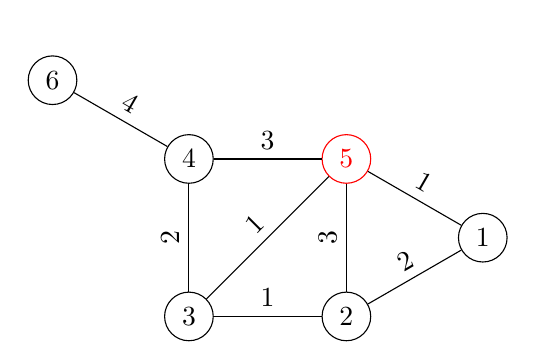
\begin{tikzpicture}[node distance=2cm]
                    \node[circle, draw] (1) {1};
                    \node[circle, draw] (2) at ([shift=(210:2)] 1) {2};
                    \node[circle, draw] (3) [left of=2] {3};
                    \node[circle, draw] (4) [above of=3] {4};
                    \node[circle, draw, red] (5) [above of=2] {5};
                    \node[circle, draw] (6) at ([shift=(150:2)] 4) {6};
    
                    \draw  (1) -- (2) node[midway, above, sloped] {2};
                    \draw (1) -- (5) node[midway, above, sloped] {1};
                    \draw (2) -- (3) node[midway, above, sloped] {1};
                    \draw (2) -- (5) node[midway, above, sloped] {3};
                    \draw (3) -- (4) node[midway, above, sloped] {2};
                    \draw (4) -- (5) node[midway, above, sloped] {3};
                    \draw (4) -- (6) node[midway, above, sloped] {4};
                    \draw (5) -- (3) node[midway, above, sloped] {1};
                \end{tikzpicture}
                \caption{Graph illustration for the highest degree vertex}
                \label{fig:vertex-highest-degree}
            \end{figure}
        \end{minipage}
        \begin{minipage}{0.5\textwidth}
            \begin{figure}[H]
                \centering
                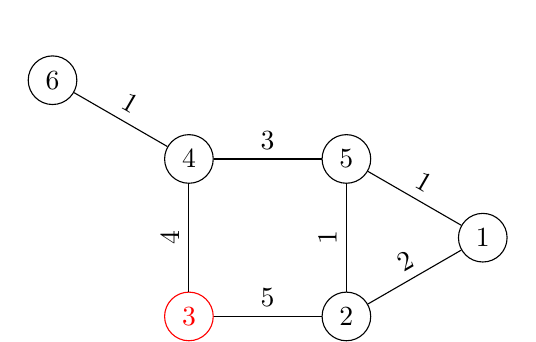
\begin{tikzpicture}[node distance=2cm]
                    \node[circle, draw] (1) {1};
                    \node[circle, draw] (2) at ([shift=(210:2)] 1) {2};
                    \node[circle, draw, red] (3) [left of=2] {3};
                    \node[circle, draw] (4) [above of=3] {4};
                    \node[circle, draw] (5) [above of=2] {5};
                    \node[circle, draw] (6) at ([shift=(150:2)] 4) {6};
    
                    \draw  (1) -- (2) node[midway, above, sloped] {2};
                    \draw (1) -- (5) node[midway, above, sloped] {1};
                    \draw (2) -- (3) node[midway, above, sloped] {5};
                    \draw (2) -- (5) node[midway, above, sloped] {1};
                    \draw (3) -- (4) node[midway, above, sloped] {4};
                    \draw (4) -- (5) node[midway, above, sloped] {3};
                    \draw (4) -- (6) node[midway, above, sloped] {1};
                \end{tikzpicture}
                \caption{Graph illustration for the vertex with the highest sum of weights of the edges}
                \label{fig:vertex-best-sum-weight-edge}
            \end{figure}
        \end{minipage}
    \end{minipage}

    \vspace{1\baselineskip}

    We implemented both ideas and performed tests on a number of graph to see which was the most consistent and we concluded that it was the vertex with the highest sum of weights of the edges. Moreover, in most graphs (at least the randomly generated ones), we had, in general, a rather homogeneous weights of edges which worked better with this one.
    \\ \\
    Constructive heuristic can be contrasted with other types of heuristics, such as local search heuristics, which try to find a solution by making small changes to an existing solution, or random heuristics, which generate solutions randomly and then choose the best one. Constructive heuristics are often used when it is important to find a solution that is complete and comprehensive, rather than just a local improvement.
    \\ \\
    Examples of some famous problems that are solved using constructive heuristics are the flow shop scheduling, the vehicle routing problem and the open shop problem.
    
    
% ----- Fonctionnement -----

\subsection{How it works}

    To explain how our algorithm works, we will keeps track of two groups of vertices : $S$ which is a partially constructed (non-maximal) clique and the partial solution that we will gradually implement. Moreover, we got $P$  which is the candidates vertices that could be included in the clique, and which represents the union of all vertex neighbors of the vertices in $S$. Furthermore, we got $W$ which is the total weight of $S$ that we will implement
    \\ \\
    The algorithm begins by identifying the vertex with the highest sum of weights of its edges. If there are multiple vertices with the same maximum sum, the vertex with the highest degree is selected. The selected vertex is then added to $S$ and its neighbors are added to $P$. Then the algorithm selects a new vertex from the candidates set $P$ and adds it to $S$. We add to $W$ the weight of the edge between the new vertex selected and every vertices in $S$. This selected vertex is the one with the most weighted edge among all the vertices in $P$. After this step, $P$ is updated by considering only the neighbors of the vertices that are already part of $S$, and by excluding the vertices that are already part of $S$ from $P$. This process is then repeated until no more vertices are left in $P$, at which point the algorithm has obtained its maximum clique $S$.
    \\ \\
    To illustrate the Constructive algorithm, let's use the example in
    Figure \ref{fig:basic-graph-example} on page \pageref{fig:basic-graph-example} while adding some weight to its edges: \\

    \begin{minipage}{\linewidth}
        \textbf{Step 0:} \newline
        \begin{minipage}{0.4\textwidth}
            \begin{figure}[H]
                \centering
                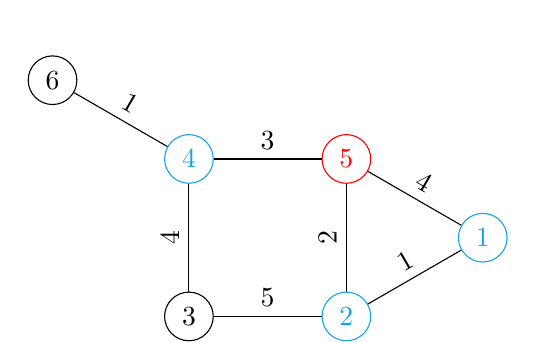
\begin{tikzpicture}[node distance=2cm]
                    \node[circle, draw, Cerulean] (1) {1};
                    \node[circle, draw, Cerulean] (2) at ([shift=(210:2)] 1) {2};
                    \node[circle, draw] (3) [left of=2] {3};
                    \node[circle, draw, Cerulean] (4) [above of=3] {4};
                    \node[circle, draw, red] (5) [above of=2] {5};
                    \node[circle, draw] (6) at ([shift=(150:2)] 4) {6};
    
                    \draw  (1) -- (2) node[midway, above, sloped] {1};
                    \draw (1) -- (5) node[midway, above, sloped] {4};
                    \draw (2) -- (3) node[midway, above, sloped] {5};
                    \draw (2) -- (5) node[midway, above, sloped] {2};
                    \draw (3) -- (4) node[midway, above, sloped] {4};
                    \draw (4) -- (5) node[midway, above, sloped] {3};
                    \draw (4) -- (6) node[midway, above, sloped] {1};
                \end{tikzpicture}
                \caption{Graph illustration for the constructive algorithm at step 0}
                \label{fig:constructive-mewc-edge}
            \end{figure}
        \end{minipage}
        \begin{minipage}{0.6\textwidth}
            At the initial step, as said before, we will initialize $S$, $P$ and $W$ by searching for the vertex with highest sum of weights of its edges $v$ by iterating every vertex on the graph. In this example, we will eventually find 3 and 5 which have a maximum sum of 9. The algorithm will then take the vertex of highest degree between them and will add it to $S$, represented in \textcolor{red}{red}. The neighboring vertex of $v$ will be added to $P$, represented in \textcolor{Cerulean}{blue}.
    
            \begin{center}
                \begin{tabular}{|lll|}
                    \hline
                    S = \{5\} & P = \{1,2,4\} & W = 0 \\
                    \hline
                \end{tabular}
            \end{center}
        \end{minipage}
    \end{minipage} 
    
    \vspace{1\baselineskip}

    \begin{minipage}{\linewidth}
        \textbf{Step 1:} \newline
        \begin{minipage}{0.4\textwidth}
            \begin{figure}[H]
                \centering
                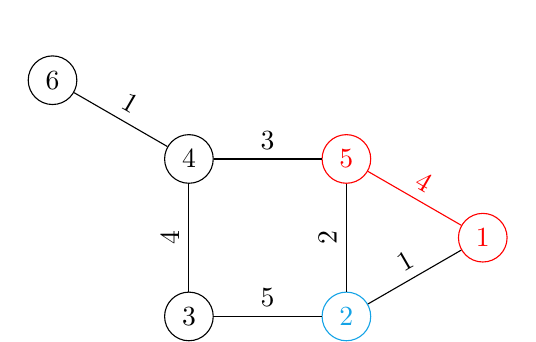
\begin{tikzpicture}[node distance=2cm]
                    \node[circle, draw, red] (1) {1};
                    \node[circle, draw, Cerulean] (2) at ([shift=(210:2)] 1) {2};
                    \node[circle, draw] (3) [left of=2] {3};
                    \node[circle, draw] (4) [above of=3] {4};
                    \node[circle, draw, red] (5) [above of=2] {5};
                    \node[circle, draw] (6) at ([shift=(150:2)] 4) {6};
    
                    \draw  (1) -- (2) node[midway, above, sloped] {1};
                    \draw[red] (1) -- (5) node[midway, above, sloped] {4};
                    \draw (2) -- (3) node[midway, above, sloped] {5};
                    \draw (2) -- (5) node[midway, above, sloped] {2};
                    \draw (3) -- (4) node[midway, above, sloped] {4};
                    \draw (4) -- (5) node[midway, above, sloped] {3};
                    \draw (4) -- (6) node[midway, above, sloped] {1};
                \end{tikzpicture}
                \caption{Graph illustration for the constructive algorithm at step 1}
                \label{fig:constructive-mewc-edge}
            \end{figure}
        \end{minipage}
        \begin{minipage}{0.6\textwidth}
            Then the algorithm will iterate all the neighbors of $v$, and look for the one who shares the edge with the highest weight, which replace $v$ (here 1). If there are several edges with the same weight, the algorithm will take the one with the highest degree. After having found it, we add it to $S$ as well as the weight of the edges of all the vertices in S and $v$ to $W$ (here 4), we update $P$ by keeping only the common neighbors of the members of $S$ (here only 2).
    
            \begin{center}
                \begin{tabular}{|lll|}
                    \hline
                    S = \{5,1\} & P = \{2\} & W = 4 \\
                    \hline
                \end{tabular}
            \end{center}
        \end{minipage}
    \end{minipage} 

    \vspace{1\baselineskip}

    \begin{minipage}{\linewidth}
        \textbf{Step 2:} \newline
        \begin{minipage}{0.4\textwidth}
            \begin{figure}[H]
                \centering
                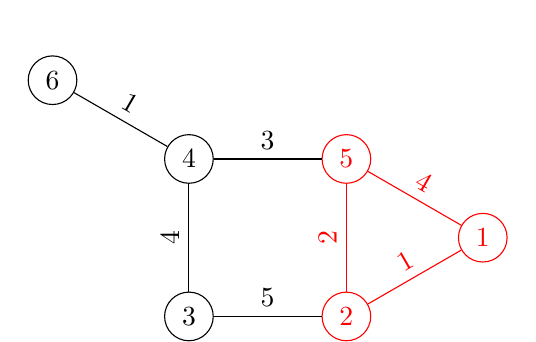
\begin{tikzpicture}[node distance=2cm]
                    \node[circle, draw, red] (1) {1};
                    \node[circle, draw, red] (2) at ([shift=(210:2)] 1) {2};
                    \node[circle, draw] (3) [left of=2] {3};
                    \node[circle, draw] (4) [above of=3] {4};
                    \node[circle, draw, red] (5) [above of=2] {5};
                    \node[circle, draw] (6) at ([shift=(150:2)] 4) {6};
    
                    \draw[red]  (1) -- (2) node[midway, above, sloped] {1};
                    \draw[red] (1) -- (5) node[midway, above, sloped] {4};
                    \draw (2) -- (3) node[midway, above, sloped] {5};
                    \draw[red] (2) -- (5) node[midway, above, sloped] {2};
                    \draw (3) -- (4) node[midway, above, sloped] {4};
                    \draw (4) -- (5) node[midway, above, sloped] {3};
                    \draw (4) -- (6) node[midway, above, sloped] {1};
                \end{tikzpicture}
                \caption{Graph illustration for the constructive algorithm at step 2}
                \label{fig:constructive-mewc-edge}
            \end{figure}
        \end{minipage}
        \begin{minipage}{0.6\textwidth}
            Then, the algorithm will repeat the process of step 1 until $P$ is empty. It will look for a new $v$ (here 2). After finding it, it will add it to $S$ as well as the weight of the edges of all the vertices in $S$ and it to $W$ (here 2 + 1). It will then update $P$ which here will be empty, the algorithm stops and we get the maximum clique in \textcolor{red}{red} and his weight (here (5,1,2) of weight 7).
    
            \begin{center}
                \begin{tabular}{|lll|}
                    \hline
                    S = \{5,1,2\} & P = \{\} & W = 7 \\
                    \hline
                \end{tabular}
            \end{center}
        \end{minipage}
    \end{minipage}

    \vspace{1\baselineskip}

    The constructive algorithm is now finished and we have obtained the following maximum clique of weight 7 : $$(1,2,5)$$

\newpage


% ----- Pseudo - Code -----

\subsection{Pseudo code}
\subsection{Complexity}

Let be a graph $G=(V,E)$ such that $n=|V|$ and $m=|E|$, we can now calculate the
complexity of our algorithm. The cost of attributing a value to a variable should
always be $\mathcal{O}(1)$. \newline

The worst case complexity of the Bron-Kerbosch algorithm is $\mathcal{O}(3^{\frac{n}{3}})$,
we will not prove it here, but it is a well-known fact proven by Moon \& Moser
\cite{on-cliques-in-graphs} that there are at most $3^{\frac{n}{3}}$ maximal cliques
in any $n$-vertex graph. \newline

The complexity of the weight calculation is $\mathcal{O}(n^2)$, because we need
to iterate two times over the vertices of the clique to get every edge and by
extension their cumulative weight. \newline

The complexity of the algorithm is therefore $\mathcal{O}(n^2\times3^{\frac{n}{3}})$,
as we need to iterate through the computed maximal cliques by the Bron-Kerbosch
algorithm and calculate their weight. \newline

The implementation of the algorithm done with efficient data structures permit us
to have a complexity of set insertion, deletion and lookup to be constant in average.

\subsection{Bad Instance}

The exact algorithm will always find the optimal solution, so it is not possible to
find a bad instance for this algorithm. However, it takes a long time to compute the
solution for large-scale graphs, so it is not feasible for large-scale graphs.
% ----- Experiments -----

\subsection{Experiments}

\begin{figure}[H]
    \centering
    \begin{tikzpicture}
        \begin{axis}[
                xlabel = Number of vertices,
                ylabel = Execution time ($\mu$s),
                legend pos = outer north east,
                grid = major,
                width = 0.7\textwidth,
            ]
            \addplot[Red, error bars/.cd, y dir=both, y explicit]
            table[x index=0, y index=1, y error index=2] {experiment_data/local_search_75_avg.dat};

            \addplot[Green, error bars/.cd, y dir=both, y explicit]
            table[x index=0, y index=1, y error index=2] {experiment_data/local_search_50_avg.dat};

            \addplot[Blue, error bars/.cd, y dir=both, y explicit]
            table[x index=0, y index=1, y error index=2] {experiment_data/local_search_25_avg.dat};

            \addplot[Black, domain=0:1000]{0.00000007146*x^5};

            \addlegendentry{test}

            \legend{75\%, 50\%, 25\%, theoretical}
        \end{axis}
    \end{tikzpicture}
    \caption{Execution time of the local search algorithm for different percentages of connectivity.}
    \label{fig:local_search_time}
\end{figure}

For this experiment, we generated five random graphs with 100 to 1000 vertices to find an average execution time for each percentage of connectivity. The connectivity is the percentage of chance that 2 vertices are linked. The results are shown in figure \ref{fig:local_search_time}. At each number of vertices, an average execution time is calculated, and the standard deviation is represented by the error bars. The number of graphs generated for each percentage of connectivity and number of vertices is limited to 5 to reduce the execution time of the experiment which already takes more than 8 minutes to compute only one result for 1000 vertices case for the 75\% connectivity. Moreover, we use a linear scale that allows us to highlight the results we want to analyze.
% ----- Analyse -----

\subsection{Analysis}

With the figure \ref{fig:grasp_time}, we can comfirm the complexity O(n^6) we found in the complexity part.
Moreover we can see some 








% ----- Local Search Algorithm -----

% ----- Local Search Algorithm -----

\section{Local Search Algorithm}

% ----- Presentation -----

\subsection{Presentation}

    A \textbf{heuristic algorithm} is a type of algorithm that uses rules of thumb to try to find an approximate solution to a problem, rather than an exact one. Heuristic algorithms are often used when it is not possible to find an exact solution to a problem, or when an exact solution would be too time-consuming to compute. They are also used when an approximate solution is good enough, or when finding an exact solution is not the primary goal. Heuristic algorithms are commonly used in artificial intelligence, computer science, and other fields. They are often used to solve optimization problems, search problems, and other types of problems where an exact solution is not necessary or practical.
    \\ \\
    A \textbf{constructive heuristic} algorithm is a type of heuristic algorithm that is used to find a solution to a problem by building it incrementally. Constructive heuristics start with a partial solution and gradually add to it until a complete solution is found. They are commonly used to solve optimization problems, where the goal is to find the optimal solution, or the solution that is the best among all possible solutions.
    \\ \\
    As we said, the use of the constructive heuristic in solving the MEWC start with a partial solution and build it until a complete solution is found. To do this, the latter will be subject to a number of criteria. 

    \begin{enumerate}
        \item Add The First Vertex to solution.
        \item Seek for his most weighted neighbors. And add it to solution if it's a neighbor of all vertices in solution.
        \item Repeat the step 2 until no vertices is available to add
    \end{enumerate}

    In these choices of criteria, we can notice one that is quite important. The one to choose the First Vertex. Indeed, it is him which will define the quality of our solution. Taking it randomly would be useless and counter productive for the sake of solving MEWC. As it was important, we thought about how to choose it and 2 answers appeared to us and we have a debate on the subject because we could not reach a consensus on it. We hesitated between these two solutions:

    \begin{itemize}
        \item The first idea was to take the highest degree vertex of the graph given as input. 
        \begin{itemize}
            \item One reason to choose the highest degree vertex as the first vertex in the solution is that it may be more likely to be part of a maximum edge weight clique(because it's the case where it's the most likely to have the biggest clique who could be the MEWC). This is because it will allow more edges to be added to the solution, which can increase the overall sum of edge weights in the clique.
            \item Another reason is that it may be more likely to be connected to other high degree vertices. This means that by adding the highest degree vertex to the clique first, we may be able to include other high degree vertices in the clique as well, which can further increase the overall sum of edge weights.
        \end{itemize}
        \item The second one was to take the vertex with the highest sum of weights of the edges.
        \begin{itemize}
            \item One reason to choose the vertex with the highest edge weight as the first vertex in the clique is that it may be more likely to be part of a maximum edge weight clique. This is because adding a vertex with a high edge weight to the clique will contribute more to the overall sum of edge weights in the clique, which is what we are trying to maximize.
            \item Another reason is that we can potentially reduce the search space for the rest of the algorithm. This is because we know that any clique we find must include this vertex, which means that we can eliminate any vertices that are not connected to it as potential members of the clique. This can help to make the algorithm more efficient by reducing the number of vertices that we need to consider.
        \end{itemize}
    \end{itemize}
    
    We will illustrate these explanations with figure 11 and 12 which shows the advantages of each over the other.
    \\ \\
    \begin{minipage}{\linewidth}
        \begin{minipage}{0.5\textwidth}
            \begin{figure}[H]
                \centering
                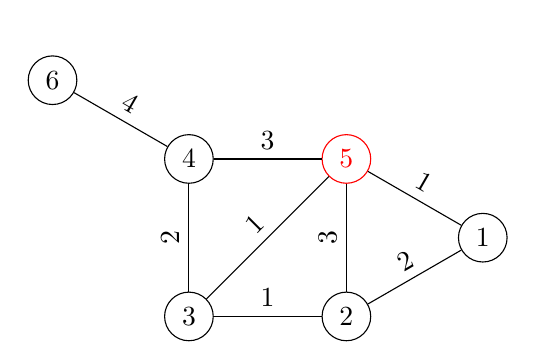
\begin{tikzpicture}[node distance=2cm]
                    \node[circle, draw] (1) {1};
                    \node[circle, draw] (2) at ([shift=(210:2)] 1) {2};
                    \node[circle, draw] (3) [left of=2] {3};
                    \node[circle, draw] (4) [above of=3] {4};
                    \node[circle, draw, red] (5) [above of=2] {5};
                    \node[circle, draw] (6) at ([shift=(150:2)] 4) {6};
    
                    \draw  (1) -- (2) node[midway, above, sloped] {2};
                    \draw (1) -- (5) node[midway, above, sloped] {1};
                    \draw (2) -- (3) node[midway, above, sloped] {1};
                    \draw (2) -- (5) node[midway, above, sloped] {3};
                    \draw (3) -- (4) node[midway, above, sloped] {2};
                    \draw (4) -- (5) node[midway, above, sloped] {3};
                    \draw (4) -- (6) node[midway, above, sloped] {4};
                    \draw (5) -- (3) node[midway, above, sloped] {1};
                \end{tikzpicture}
                \caption{Graph illustration for the highest degree vertex}
                \label{fig:vertex-highest-degree}
            \end{figure}
        \end{minipage}
        \begin{minipage}{0.5\textwidth}
            \begin{figure}[H]
                \centering
                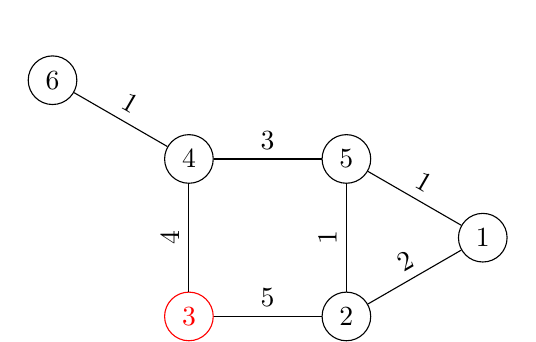
\begin{tikzpicture}[node distance=2cm]
                    \node[circle, draw] (1) {1};
                    \node[circle, draw] (2) at ([shift=(210:2)] 1) {2};
                    \node[circle, draw, red] (3) [left of=2] {3};
                    \node[circle, draw] (4) [above of=3] {4};
                    \node[circle, draw] (5) [above of=2] {5};
                    \node[circle, draw] (6) at ([shift=(150:2)] 4) {6};
    
                    \draw  (1) -- (2) node[midway, above, sloped] {2};
                    \draw (1) -- (5) node[midway, above, sloped] {1};
                    \draw (2) -- (3) node[midway, above, sloped] {5};
                    \draw (2) -- (5) node[midway, above, sloped] {1};
                    \draw (3) -- (4) node[midway, above, sloped] {4};
                    \draw (4) -- (5) node[midway, above, sloped] {3};
                    \draw (4) -- (6) node[midway, above, sloped] {1};
                \end{tikzpicture}
                \caption{Graph illustration for the vertex with the highest sum of weights of the edges}
                \label{fig:vertex-best-sum-weight-edge}
            \end{figure}
        \end{minipage}
    \end{minipage}

    \vspace{1\baselineskip}

    We implemented both ideas and performed tests on a number of graph to see which was the most consistent and we concluded that it was the vertex with the highest sum of weights of the edges. Moreover, in most graphs (at least the randomly generated ones), we had, in general, a rather homogeneous weights of edges which worked better with this one.
    \\ \\
    Constructive heuristic can be contrasted with other types of heuristics, such as local search heuristics, which try to find a solution by making small changes to an existing solution, or random heuristics, which generate solutions randomly and then choose the best one. Constructive heuristics are often used when it is important to find a solution that is complete and comprehensive, rather than just a local improvement.
    \\ \\
    Examples of some famous problems that are solved using constructive heuristics are the flow shop scheduling, the vehicle routing problem and the open shop problem.
    
    
% ----- Fonctionnement -----

\subsection{How it works}

    To explain how our algorithm works, we will keeps track of two groups of vertices : $S$ which is a partially constructed (non-maximal) clique and the partial solution that we will gradually implement. Moreover, we got $P$  which is the candidates vertices that could be included in the clique, and which represents the union of all vertex neighbors of the vertices in $S$. Furthermore, we got $W$ which is the total weight of $S$ that we will implement
    \\ \\
    The algorithm begins by identifying the vertex with the highest sum of weights of its edges. If there are multiple vertices with the same maximum sum, the vertex with the highest degree is selected. The selected vertex is then added to $S$ and its neighbors are added to $P$. Then the algorithm selects a new vertex from the candidates set $P$ and adds it to $S$. We add to $W$ the weight of the edge between the new vertex selected and every vertices in $S$. This selected vertex is the one with the most weighted edge among all the vertices in $P$. After this step, $P$ is updated by considering only the neighbors of the vertices that are already part of $S$, and by excluding the vertices that are already part of $S$ from $P$. This process is then repeated until no more vertices are left in $P$, at which point the algorithm has obtained its maximum clique $S$.
    \\ \\
    To illustrate the Constructive algorithm, let's use the example in
    Figure \ref{fig:basic-graph-example} on page \pageref{fig:basic-graph-example} while adding some weight to its edges: \\

    \begin{minipage}{\linewidth}
        \textbf{Step 0:} \newline
        \begin{minipage}{0.4\textwidth}
            \begin{figure}[H]
                \centering
                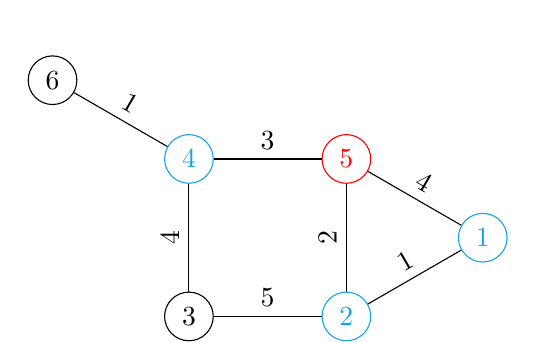
\begin{tikzpicture}[node distance=2cm]
                    \node[circle, draw, Cerulean] (1) {1};
                    \node[circle, draw, Cerulean] (2) at ([shift=(210:2)] 1) {2};
                    \node[circle, draw] (3) [left of=2] {3};
                    \node[circle, draw, Cerulean] (4) [above of=3] {4};
                    \node[circle, draw, red] (5) [above of=2] {5};
                    \node[circle, draw] (6) at ([shift=(150:2)] 4) {6};
    
                    \draw  (1) -- (2) node[midway, above, sloped] {1};
                    \draw (1) -- (5) node[midway, above, sloped] {4};
                    \draw (2) -- (3) node[midway, above, sloped] {5};
                    \draw (2) -- (5) node[midway, above, sloped] {2};
                    \draw (3) -- (4) node[midway, above, sloped] {4};
                    \draw (4) -- (5) node[midway, above, sloped] {3};
                    \draw (4) -- (6) node[midway, above, sloped] {1};
                \end{tikzpicture}
                \caption{Graph illustration for the constructive algorithm at step 0}
                \label{fig:constructive-mewc-edge}
            \end{figure}
        \end{minipage}
        \begin{minipage}{0.6\textwidth}
            At the initial step, as said before, we will initialize $S$, $P$ and $W$ by searching for the vertex with highest sum of weights of its edges $v$ by iterating every vertex on the graph. In this example, we will eventually find 3 and 5 which have a maximum sum of 9. The algorithm will then take the vertex of highest degree between them and will add it to $S$, represented in \textcolor{red}{red}. The neighboring vertex of $v$ will be added to $P$, represented in \textcolor{Cerulean}{blue}.
    
            \begin{center}
                \begin{tabular}{|lll|}
                    \hline
                    S = \{5\} & P = \{1,2,4\} & W = 0 \\
                    \hline
                \end{tabular}
            \end{center}
        \end{minipage}
    \end{minipage} 
    
    \vspace{1\baselineskip}

    \begin{minipage}{\linewidth}
        \textbf{Step 1:} \newline
        \begin{minipage}{0.4\textwidth}
            \begin{figure}[H]
                \centering
                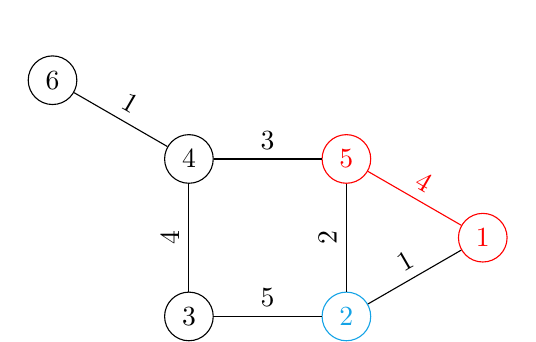
\begin{tikzpicture}[node distance=2cm]
                    \node[circle, draw, red] (1) {1};
                    \node[circle, draw, Cerulean] (2) at ([shift=(210:2)] 1) {2};
                    \node[circle, draw] (3) [left of=2] {3};
                    \node[circle, draw] (4) [above of=3] {4};
                    \node[circle, draw, red] (5) [above of=2] {5};
                    \node[circle, draw] (6) at ([shift=(150:2)] 4) {6};
    
                    \draw  (1) -- (2) node[midway, above, sloped] {1};
                    \draw[red] (1) -- (5) node[midway, above, sloped] {4};
                    \draw (2) -- (3) node[midway, above, sloped] {5};
                    \draw (2) -- (5) node[midway, above, sloped] {2};
                    \draw (3) -- (4) node[midway, above, sloped] {4};
                    \draw (4) -- (5) node[midway, above, sloped] {3};
                    \draw (4) -- (6) node[midway, above, sloped] {1};
                \end{tikzpicture}
                \caption{Graph illustration for the constructive algorithm at step 1}
                \label{fig:constructive-mewc-edge}
            \end{figure}
        \end{minipage}
        \begin{minipage}{0.6\textwidth}
            Then the algorithm will iterate all the neighbors of $v$, and look for the one who shares the edge with the highest weight, which replace $v$ (here 1). If there are several edges with the same weight, the algorithm will take the one with the highest degree. After having found it, we add it to $S$ as well as the weight of the edges of all the vertices in S and $v$ to $W$ (here 4), we update $P$ by keeping only the common neighbors of the members of $S$ (here only 2).
    
            \begin{center}
                \begin{tabular}{|lll|}
                    \hline
                    S = \{5,1\} & P = \{2\} & W = 4 \\
                    \hline
                \end{tabular}
            \end{center}
        \end{minipage}
    \end{minipage} 

    \vspace{1\baselineskip}

    \begin{minipage}{\linewidth}
        \textbf{Step 2:} \newline
        \begin{minipage}{0.4\textwidth}
            \begin{figure}[H]
                \centering
                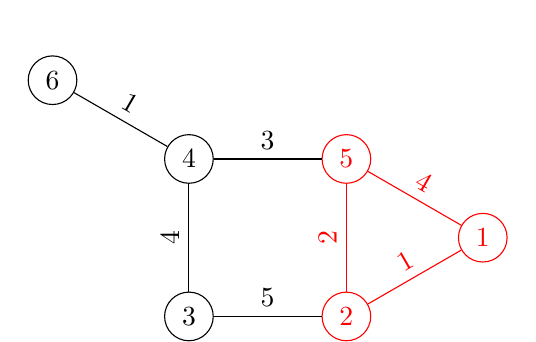
\begin{tikzpicture}[node distance=2cm]
                    \node[circle, draw, red] (1) {1};
                    \node[circle, draw, red] (2) at ([shift=(210:2)] 1) {2};
                    \node[circle, draw] (3) [left of=2] {3};
                    \node[circle, draw] (4) [above of=3] {4};
                    \node[circle, draw, red] (5) [above of=2] {5};
                    \node[circle, draw] (6) at ([shift=(150:2)] 4) {6};
    
                    \draw[red]  (1) -- (2) node[midway, above, sloped] {1};
                    \draw[red] (1) -- (5) node[midway, above, sloped] {4};
                    \draw (2) -- (3) node[midway, above, sloped] {5};
                    \draw[red] (2) -- (5) node[midway, above, sloped] {2};
                    \draw (3) -- (4) node[midway, above, sloped] {4};
                    \draw (4) -- (5) node[midway, above, sloped] {3};
                    \draw (4) -- (6) node[midway, above, sloped] {1};
                \end{tikzpicture}
                \caption{Graph illustration for the constructive algorithm at step 2}
                \label{fig:constructive-mewc-edge}
            \end{figure}
        \end{minipage}
        \begin{minipage}{0.6\textwidth}
            Then, the algorithm will repeat the process of step 1 until $P$ is empty. It will look for a new $v$ (here 2). After finding it, it will add it to $S$ as well as the weight of the edges of all the vertices in $S$ and it to $W$ (here 2 + 1). It will then update $P$ which here will be empty, the algorithm stops and we get the maximum clique in \textcolor{red}{red} and his weight (here (5,1,2) of weight 7).
    
            \begin{center}
                \begin{tabular}{|lll|}
                    \hline
                    S = \{5,1,2\} & P = \{\} & W = 7 \\
                    \hline
                \end{tabular}
            \end{center}
        \end{minipage}
    \end{minipage}

    \vspace{1\baselineskip}

    The constructive algorithm is now finished and we have obtained the following maximum clique of weight 7 : $$(1,2,5)$$

\newpage


% ----- Pseudo - Code -----

\subsection{Pseudo code}
\subsection{Complexity}

Let be a graph $G=(V,E)$ such that $n=|V|$ and $m=|E|$, we can now calculate the
complexity of our algorithm. The cost of attributing a value to a variable should
always be $\mathcal{O}(1)$. \newline

The worst case complexity of the Bron-Kerbosch algorithm is $\mathcal{O}(3^{\frac{n}{3}})$,
we will not prove it here, but it is a well-known fact proven by Moon \& Moser
\cite{on-cliques-in-graphs} that there are at most $3^{\frac{n}{3}}$ maximal cliques
in any $n$-vertex graph. \newline

The complexity of the weight calculation is $\mathcal{O}(n^2)$, because we need
to iterate two times over the vertices of the clique to get every edge and by
extension their cumulative weight. \newline

The complexity of the algorithm is therefore $\mathcal{O}(n^2\times3^{\frac{n}{3}})$,
as we need to iterate through the computed maximal cliques by the Bron-Kerbosch
algorithm and calculate their weight. \newline

The implementation of the algorithm done with efficient data structures permit us
to have a complexity of set insertion, deletion and lookup to be constant in average.

\subsection{Bad Instance}

The exact algorithm will always find the optimal solution, so it is not possible to
find a bad instance for this algorithm. However, it takes a long time to compute the
solution for large-scale graphs, so it is not feasible for large-scale graphs.
% ----- Experiments -----

\subsection{Experiments}

\begin{figure}[H]
    \centering
    \begin{tikzpicture}
        \begin{axis}[
                xlabel = Number of vertices,
                ylabel = Execution time ($\mu$s),
                legend pos = outer north east,
                grid = major,
                width = 0.7\textwidth,
            ]
            \addplot[Red, error bars/.cd, y dir=both, y explicit]
            table[x index=0, y index=1, y error index=2] {experiment_data/local_search_75_avg.dat};

            \addplot[Green, error bars/.cd, y dir=both, y explicit]
            table[x index=0, y index=1, y error index=2] {experiment_data/local_search_50_avg.dat};

            \addplot[Blue, error bars/.cd, y dir=both, y explicit]
            table[x index=0, y index=1, y error index=2] {experiment_data/local_search_25_avg.dat};

            \addplot[Black, domain=0:1000]{0.00000007146*x^5};

            \addlegendentry{test}

            \legend{75\%, 50\%, 25\%, theoretical}
        \end{axis}
    \end{tikzpicture}
    \caption{Execution time of the local search algorithm for different percentages of connectivity.}
    \label{fig:local_search_time}
\end{figure}

For this experiment, we generated five random graphs with 100 to 1000 vertices to find an average execution time for each percentage of connectivity. The connectivity is the percentage of chance that 2 vertices are linked. The results are shown in figure \ref{fig:local_search_time}. At each number of vertices, an average execution time is calculated, and the standard deviation is represented by the error bars. The number of graphs generated for each percentage of connectivity and number of vertices is limited to 5 to reduce the execution time of the experiment which already takes more than 8 minutes to compute only one result for 1000 vertices case for the 75\% connectivity. Moreover, we use a linear scale that allows us to highlight the results we want to analyze.
% ----- Analyse -----

\subsection{Analysis}

With the figure \ref{fig:grasp_time}, we can comfirm the complexity O(n^6) we found in the complexity part.
Moreover we can see some 








% ----- Grasp Algorithm -----

% ----- Grasp Algorithm -----

\section{Grasp Algorithm}

% ----- Presentation -----

\subsection{Presentation}

% ----- Fonctionnement -----

\subsection{How it works}

% ----- Pseudo - Code -----

\subsection{Pseudo code}

% ----- Complexité -----

\subsection{Complexity}

% ----- Instance -----

\subsection{Instance}

% ----- Experiments -----

\subsection{Experiments}

% ----- Analyse -----

\subsection{Analysis}


% ----- Conclusion -----

% ----- Conclusion -----

\section{Conclusion}

As we have seen before, the MEWC problem is a problem that we cannot answer for a general case. 
As these algorithms are NP-hard we cannot find a solution in polynomial time.
By trying to optimize the solution of the problem we notice that the algorithms are more or less efficient depending on different criteria which are :

\begin{itemize}
    \item \textbf{The number of vertices} 

    \item \textbf{The connectivity of them}

    \item \textbf{The random generation} which can create special cases for some algorithms (bad instances)
\end{itemize}

We can therefore deduce from the graph (the one to study) that we can select the most suitable algorithm to solve the problem in the best way.\bigskip

\large\textbf{Comparison of algorithms} \newline 

\underline{Speed of results}\bigskip

We are now going to compare the different algorithms from a general point of view, even if it would be necessary to do a study again according to the starting graph we have.
Let's look at the complexity and the execution time of these different algorithms.

\begin{itemize}
    \item \textbf{Complexity} : As we compare the complexity of the algorithms we obtain : \bigskip
    
Exact (O($n^2\sqrt[3]{3}^n$)) - Constructive (O($n^2$)) - Local Search (O($n^5$)) - Grasp (O($n^6$)) \bigskip
    
    Since the complexity will vary depending on the connectivity and degeneracy of the graph we will look at the execution time too.
    
    \item \textbf{Execution time} : \bigskip
    
Constructive ($5.10^6$) -  Local Search (A COMPLETER) - Grasp ($10^8$) - Exact ($\thicksim 10^8$) 
\end{itemize}
\underline{Accuracy of results}\bigskip 

Another very important criterion to consider is the accuracy of the answer obtained. \bigskip 

Accuracy is in this order (from most to least accurate):

Exact - Grasp - Local Search - Constructive \bigskip 

\large\textbf{Choice of the algorithm} \newline

After this, we decided to conclude according to the number of vertices of our strating graph :

\begin{itemize}
    \item \textbf{10 - 100 Vertices} : We will use the "Exact" algorithm which allows to give a very precise solution but which is slow.

    \item \textbf{100 + Vertices} : In order to don't wait too long for an answer, we plan to use the "Grasp" algorithm and then the "Local Search" which are certainly less precise but which allows to give an answer in less time.

    \item \textbf{5000 + Vertices} : Finally we will use the "Constructive" algorithm which is the least precise but the fastest and allows to answer in an acceptable time

\end{itemize}

\begin{figure}[H]
    \centering
    \begin{tikzpicture}
        \begin{axis}[
                xlabel = Number of vertices,
                ylabel = \% of solution based on exact,
                legend pos = outer north east,
                grid = major,
                width = 0.5\textwidth,
                legend cell align = {left},
            ]
            \addplot[Red, error bars/.cd, y dir=both, y explicit]
            table[x index=0, y index=1] {experiment_data/accuracy_avg_exact.dat};

            \addplot[Green, error bars/.cd, y dir=both, y explicit]
            table[x index=0, y index=1] {experiment_data/accuracy_avg_constructive_25.dat};

            \addplot[Blue, error bars/.cd, y dir=both, y explicit]
            table[x index=0, y index=1] {experiment_data/accuracy_avg_local_search_25.dat};

            \addplot[Black, error bars/.cd, y dir=both, y explicit]
            table[x index=0, y index=1] {experiment_data/accuracy_avg_grasp_25.dat};

            \addlegendentry{test}

            \legend{exact, constructive, local search, grasp}
        \end{axis}
    \end{tikzpicture}
    \caption{\% of solution based on the exact of the different algorithm for 25\% of connectivity.}
    \label{fig:algorithm_25_time}
\end{figure}

For this experiment, we generated 10 random graphs with 10 to 100 vertices to find an
average \% for 25\% of connectivity. The connectivity is the percentage
of chance that 2 vertices are linked. The results are shown in figure \ref{fig:algorithm_25_time}. At each number of
vertices, an average clique weight is calculated, and converted to \% based on the result obtained with the exact algorithm.
// à martin de détailler

\begin{figure}[H]
    \centering
    \begin{tikzpicture}
        \begin{axis}[
            xlabel = Number of vertices,
            ylabel = \% of solution based on exact,
                legend pos = outer north east,
                grid = major,
                width = 0.5\textwidth,
                legend cell align = {left},
            ]
            \addplot[Red, error bars/.cd, y dir=both, y explicit]
            table[x index=0, y index=1] {experiment_data/accuracy_avg_exact.dat};

            \addplot[Green, error bars/.cd, y dir=both, y explicit]
            table[x index=0, y index=1] {experiment_data/accuracy_avg_constructive_50.dat};

            \addplot[Blue, error bars/.cd, y dir=both, y explicit]
            table[x index=0, y index=1] {experiment_data/accuracy_avg_local_search_50.dat};

            \addplot[Black, error bars/.cd, y dir=both, y explicit]
            table[x index=0, y index=1] {experiment_data/accuracy_avg_grasp_50.dat};

            \addlegendentry{test}

            \legend{exact, constructive, local search, grasp}
        \end{axis}
    \end{tikzpicture}
    \caption{\% of solution based on the exact of the different algorithm for 50\% of connectivity.}
    \label{fig:algorithm_50_time}
\end{figure}

For this experiment, we generated 10 random graphs with 10 to 100 vertices to find an
average \% for 50\% of connectivity. The connectivity is the percentage
of chance that 2 vertices are linked. The results are shown in figure \ref{fig:algorithm_50_time}. At each number of
vertices, an average clique weight is calculated, and converted to \% based on the result obtained with the exact algorithm.
// à martin de détailler

\begin{figure}[H]
    \centering
    \begin{tikzpicture}
        \begin{axis}[
            xlabel = Number of vertices,
            ylabel = \% of solution based on the exact,
                legend pos = outer north east,
                grid = major,
                width = 0.5\textwidth,
                legend cell align = {left},
            ]
            \addplot[Red, error bars/.cd, y dir=both, y explicit]
            table[x index=0, y index=1] {experiment_data/accuracy_avg_exact.dat};

            \addplot[Green, error bars/.cd, y dir=both, y explicit]
            table[x index=0, y index=1] {experiment_data/accuracy_avg_constructive_75.dat};

            \addplot[Blue, error bars/.cd, y dir=both, y explicit]
            table[x index=0, y index=1] {experiment_data/accuracy_avg_local_search_75.dat};

            \addplot[Black, error bars/.cd, y dir=both, y explicit]
            table[x index=0, y index=1] {experiment_data/accuracy_avg_grasp_75.dat};

            \addlegendentry{test}

            \legend{exact, constructive, local search, grasp}
        \end{axis}
    \end{tikzpicture}
    \caption{\% of solution based on the exact of the different algorithm for 75\% of connectivity.}
    \label{fig:algorithm_75_time}
\end{figure}

For this experiment, we generated 10 random graphs with 10 to 100 vertices to find an
average \% of clique weight for 75\% of connectivity. The connectivity is the percentage
of chance that 2 vertices are linked. The results are shown in figure \ref{fig:algorithm_75_time}. At each number of
vertices, an average clique weight is calculated, and converted to \% based on the result obtained with the exact algorithm.
// à martin de détailler

% ----- Bibliographie -----

\bibliographystyle{plain}
\bibliography{fichier_latex/bibliographie.bib}

\end{document}